\documentclass{article}
\usepackage{amssymb}
\usepackage{amsfonts}
\usepackage{amsmath}
\usepackage{amsthm}
\usepackage{url}
\usepackage{graphicx}
\usepackage{eqlist}
\usepackage{natbib}
\usepackage{fancyvrb}
\usepackage{color}

\usepackage[table]{xcolor}

%\usepackage[perpage,symbol*]{footmisc}

%\DefineFNsymbols*{daggers}{\dagger\ddagger{\dagger\suck\dagger}{\ddagger\ddagger}*{**}{***}}
%\setfnsymbol{daggers}

 
\begin{document}
\title{$msms$ User Manual}  
\maketitle
\section{Introduction}  

This document describes how to use $msms$, a tool to generate sequence samples 
under both neutral models and a single locus selection model. $msms$ permits the
full range of demographic models provided by ms\citep{hudson_generating_2002}.
In particular, it allows for multiple demes with arbitrary migration patterns,
population growth and decay in each deme, and for population splits and
mergers. Selection (including dominance) can depend on the deme and also change
with time. The program is designed to be command line compatible to ms, however
no prior knowledge of ms is assumed for this document. 

Applications of this program include power studies, analytical comparisons,
approximated Bayesian computation among many others. Because most applications
require the generation of a large number of independent replicates, the code is
designed to be efficient and fast. For the neutral case, it is comparable to ms
and even faster for large recombination rates. For selection, the performance is
only slightly slower, making this one of the fastest tools for simulation with
selection.
 
The program has been developed with a wide number of possible operating systems
and hardware in mind. For this reason, the code has been developed in Java and
can run on any hardware that supports Java 1.6. This includes Mac OS X, all
current versions of MS Windows, and most Unix flavors (Linux, Sun, BSD). The
Java programing language is also popular and widely known which should
facilitate the writing of extensions for the program.

\subsection{Conventions}

$msms$ is a command line program and as such must be run from the shell in Unix
and Mac OS X or from a command prompt in Windows. Generally this document uses
the convention that text entered into a command line will be formatted as
follows.
\begin{verbatim}
	>java -jar msms.jar
\end{verbatim}
Here the {\tt >} denotes the command line prompt, and you do not type this, also
note that some command line prompts will be different depending on the
system\footnote{{\tt \$} is common }. The ``{\tt -}'' with the following text
is referred to as a switch. So in the above example, we call the {\tt java}
command with the {\tt -jar} switch, with the argument {\tt msms.jar}. 

Time is measured from the present into the past, and we use the term {\it
pastward}.  This is common for coalescent simulations and conforms to the
convention in ms.  Time units are always in $4N_e$ generations. The present is defined as the
time of sampling. That is when sequencing was done.\footnote{At this stage we do
not consider temporal sampling
  of populations. However if there was demand for such a feature, this could be
  easily added.}. 
  
  %Here $N_e$ is not specifically defined as the coalescent is
  %scale invariant with $N_e$ when not considering selection. Otherwise $N_e$
  %can be defined explicitly. 

\section{Installation}
All relevant files are located at \url{http://www.mabs.at/ewing/msms/}\

\subsection{Recommended}

You must have Java 6 installed. Note that this is in fact Java 1.6 so don't
worry about the different names, they are the same thing. This can be
downloaded from the sun website from \url{http://www.Java.com/en/download/}\ .
On an OSX machine, you just need to ensure you have the latest updates from Apple.
However, by default it will still use Java 5 even though you have Java 6
installed. To change this go to
\begin{verbatim}
Applications->Utilities->Java Preferences
\end{verbatim}
and ensure that Java 6 or better is ticked, and dragged to the top of all the
lists. Also, you will need to start with a fresh command line to see these
changes.

For normal installation, download the zip file and unpack to a directory of your
choice. This creates a directory called msms with some subdirectories. In
particular, you will have a bin directory that holds the binaries, or more to the
point the program launchers. You will probably want this directory added to the
path. Under Unix and OSX you can use simlinks for the {\tt msms} launching
scripts. Note that {\tt msms.exe} is for Windows machines only. 

The rest of this document assumes that the bin directory is in the path. Thus,
you only need to use {\tt msms} at the command line to invoke the program. If
this is not the case, the command line may need to be prefixed with more
options. 

\subsection{Pure jar}

We also make the program available as a jar file with the correctly configured
manifest file. To invoke the program, no installation is required other than
downloading the {\tt msms.jar} file, and then use Java with the {\tt -jar}
switch:
\begin{verbatim}
>java -jar msms.jar
\end{verbatim}
Note that this is long hand for the normal command,
\begin{verbatim}
>msms
\end{verbatim}
that we use throughout this document. Also, recall that by default Java will assume
a maximum memory size of just 64Mb. So, for some simulations the use of the
Java {\tt -Xmx} switch will be required. If you downloaded the normal package,
the {\tt msms.jar} file can be found in the lib subdirectory. 

\subsection{From Source}
The source is also provided as a downloaded zip file. This is not the
recommended option unless you wish to modify the source code. We use {\tt ant}
\url{http://ant.apache.org/} as the build tool. The {\tt build.xml} file is in
the subdirectory {\tt ant}. Please check the {\tt readme.txt} included in the
source download.

\subsection{Git}
Please check the website for instructions on the details of the git
repository.  

\section{Simple Usage and $ms$ Compatibility}

The basic command line options without selection are:
\begin{verbatim}
>msms -ms sampleCount reps -t theta 
\end{verbatim}
Here, we generate {\tt sampleCount} samples per simulation with a population size
of $N_e=${\tt popSize} and a $\theta=4N_e\mu$ of {\tt theta}. Since we are
simulating under a neutral model and all parameters are scaled relative to $N_e$,
that there is no requirement to set $N_e$. Note that the input
switches are the same as per $ms$. For example, the $ms$ command line for the
above is:
\begin{verbatim}
>ms sampleCount reps -t theta  
\end{verbatim}
In general, any $ms$ options can be run\footnote{except gene conversion} by
just changing the program.
For example the $ms$ command: 
\begin{Verbatim}[commandchars=\\\{\}]
>ms sampleCount reps -t theta  \textit{other ms switches}
\end{Verbatim}
will be run in $msms$ by:
\begin{Verbatim}[commandchars=\\\{\}]
>msms \textcolor{red}{sampleCount reps -t theta \textit{other ms switches}}
\end{Verbatim}
where the red text is the ms command line options. For this reason, the $ms$
manual provided with ms is a valuable resource, and all  examples are equally
valid for $msms$.

In previous version there was a {\tt -ms} switch that was required for $ms$
compatibility. This is no longer required, however the option can still be used. 

\subsection{Output}

After running the program the following output is generated:
\begin{verbatim}
>msms -ms 5 2 -t 1
msms 5 2 -t 1 
rnd numbers

//
segsites: 2
positions: 0.50061 0.70488
10
00
00
00
01

// 
segsites: 3 
positions: 0.11559 0.32324 0.46842
100 
000 
011 
011 
011
\end{verbatim}
In this example, we have $\theta=1$ with a sample size of 5  and 2 replicates.
The output is the same as in ms, with some subtle differences. The first line is
simply the command line with the {\tt -ms} switch omitted in order to stay
compatible with ms parsing tools. Note that we keep the arguments to the {\tt
-ms} switch as per $ms$. So, the first line is the command msms followed by the
sample size and the number of replicates. After this comes the rest of the
command line. We attempt to place ms compatible options before any $msms$
specific ones. This is in an attempt to remain compatible with some tools that
parse $ms$ output.

The next line is simply the text {\tt rnd numbers}. This is for ms tool chain
compatibility. The random number generators for $msms$ are different from ms and
hence, we do not output misleading numbers.

After this, we have a blank line followed by a line with {\tt //} denoting the
start of a sample output. The next 2 lines give us the number of segregation
sites followed by their position within the neutral locus in increasing order.
By default, the neutral locus is the interval between $0$ and $1$. However, as we
see later the user may specify multiple neutral selected loci over different
intervals. 

Finally we have 5 lines, one line for each sampled sequence, with the haplotype
information. The derived allele is denoted with a 1 and the ancestral type with a 0. These are
in the same order as in the positions list. This data is generated under the
infinite sites model. We currently do not support other neutral mutation models. 


\subsection{Recombination}

Recombination can be included in the simulation with the {\tt -r} switch, as
in the following example:
\begin{verbatim}
>msms  5 2 -t 1 -r 1 
\end{verbatim}
Here, we have a recombination rate $\rho=4N_er$ where $r$ is the probability of
recombination per generation between the ends of a unit length locus. Thus, the
recombination rate of a locus that is 2 units long will have an effective
recombination rate twice as large as a single unit locus. In this case, we 
use an infinite {\it recombination sites} model for recombination. However, if
we use the command in the following way, 
\begin{Verbatim}[commandchars=\\\{\}]
>msms 5 2 -t 1 -r 1 \textcolor{red}{1000} 
\end{Verbatim}
then we have specified a finite cut site model with 1000 recombination sites per unit
of neutral locus. Using this option can improve performance substantially over
the infinite recombination sites model when recombination is high while still
being an accurate model. 

\section{Structured Population Models}

Population structure with multiple demes is defined in the same way as in ms,
using the {\tt -I} switch.
\begin{verbatim}
-I npop sample1 sample2 ... sampleK mrate 
\end{verbatim}
The first argument {\tt npop} is the number of demes or subpopulations. Each
subpopulation has population size $N_e$ by default. The following arguments are
the sample sizes. A sample size (which can be zero) must be specified for each
deme, and the sample sizes from all demes must add up to the correct total sample
size. In the example, migration is introduced according to a simple island model
with uniform migration rate {\tt mrate} in units of $4N_em$. This corresponds to
a migration matrix with all nondiagonal entries set to $4N_em/(\texttt{npop}-1)$,
see below for more general migration schemes. The haplotype output is ordered so
that the first {\tt sample1} entries are from deme 1, the next {\tt sample2}
entries are from the second deme and so forth. Demes are labeled 1 to {\tt npop}
while both $\theta$ and the recombination rate are  always scaled to $N_e$, not
the total population size. In fact in general, all parameters are scaled to $N_e$
and can be specified with the {\tt -N} switch.

\subsection{Subpopulation Sizes}

We can also specify the population of any subpopulation individually with the
{\tt -n} switch. This switch must come after the -I switch. The arguments to
the switch are as follows:
\begin{verbatim}
-n pop scale
\end{verbatim}
Where {\tt pop} is the subpopulation deme label or index and scale is the new
size relative to $N_e$. Any number of {\tt -n} switches can be used, and if the
same population label is used in more than one, the last specified value is the
one used. 

\subsection{Migration Rates}
There are two ways to define a detailed migration model. The first method is with
the {\tt -m} switch where we can specify a single entry in the migration matrix
using the following syntax:
\begin{verbatim}
-m i j 4Nm
\end{verbatim}
where {\tt i} and {\tt j} are subpopulation labels and {\tt 4Nm} is the new
migration rate. We define  the migration matrix as follows: $M=m_{ij}\ i\neq
j;i,j \in \{1,\ldots,\texttt{npop}\}$ where $m_{ij}$ is the fraction of
subpopulation $i$ that is made up of migrants from subpopulation $j$ in forward
time. Hence pastward we have the rate that a lineage moves from deme $i$ to $j$
as $m_{ij}$. 

Alternatively, we can specify a complete migration matrix at once with the {\tt
-ma} switch. The arguments are:
\begin{verbatim}
-ma x m12 m13 m21 x m23 m31 m32 x
\end{verbatim}
where {\tt m12} is the $m_{12}$ entry of the migration matrix. The
diagonal entries are labeled with an {\tt x} but anything that aids readability
can be used, and they must be present. 

\subsubsection{Example}

In our first example, we have 2 demes where the second deme is half the size of
the first deme. Migration is twice as high in the direction of deme 1 to deme 2.
There are 6 sequences sampled from the first deme and only 4 from the last deme.
\begin{verbatim}
>msms 10 100 -t 1 -I 2 6 4 1.0 -n 2 .5 -m 1 2 2.0
\end{verbatim} 
Here, the migration rates are all set to 1.0, and then we set the $m_{12}$ entry
to 2.0. Likewise the population size of both demes is set to 10000, and then
for deme 2 it is multiplied by .5 with the {\tt -n} switch. We can write the same model
using the {\tt -ma} switch as follows:
\begin{verbatim}
>msms 10 100 -t 1 -I 2 6 4 1.0 -n 2 .5 -ma x 2.0 1.0 x
\end{verbatim} 


\newpage

\section{Introducing Selection}
\label{simpleSelection}
\subsection{Conditioning on Fixation and Frequencies}
\textcolor{red}{
\begin{center}
{\large WARNING}
\end{center}
This option can only be used with models that
are time invariant. That is, the model can not change over time. This means you
cannot use this option if you use any of the switches that start with {\tt -e}
such as {\tt -ej -ema -es -en}. }
\ \newline

We first consider the case of selection on a single allele that we assume goes
to fixation. The command line is as follows:

\begin{verbatim}
>msms -N 1000 -ms 5 2 -t 1 -r 1 -SAA sAA -SaA saA -SF time
\end{verbatim}

Alternatively we could omit the optional {\tt -ms} switch but then must reorder
command

\begin{verbatim}
>msms 5 2 -N 1000 -t 1 -r 1 -SAA sAA -SaA saA -SF time
\end{verbatim}

Here, {\tt sAA} and {\tt saA} are the selection coefficients for the
homozygote AA and heterozygote aA genotypes respectively. Selection strength is specified in
units of $2N_es$ and we define $w_{AA}=1+s_{AA}$ with $w_{AA}$ as the Malthusian
fitness. We assume diploid populations. Finally, we specify the time after the
beneficial allele went to fixation with the {\tt -SF}  switch with time
specified pastward and in units of $4N_e$ generations. In this  case, we assume a single
founder (a single beneficial mutation) has been picked up by selection. Or, in
other words we condition on a single beneficial mutation going  to fixation, and the initial
frequency of the beneficial allele is $1/2N_e$. In order for the simulations that
use {\tt -SF} switch to work, the demographic history, indeed the full model,
must be time invariant. That is,  all parameters of the model cannot change over
time. See below for the options that  permit time variant models.

When we have selection, despite the fact that all parameters are scaled to $N_e$,
the actual value becomes important. The forward simulation uses discrete
generations and a discrete population size. Thus, the run time is influenced by
how large the {\tt -N} switch is set to. Larger is generally slower. Furthermore,
the variance of the binomial sampling (drift) depends on $N_e$ and hence, the
variance between simulation runs will also depend on $N_e$. Because of its
relevance, you must specify the {\tt -N} switch when including
selection. Generally, the performance is good enough to use a realistic value for $N_e$.

Another consideration when simulating with discrete generations is accuracy
compared to continuous approximations. Generally, a very small $N_e$ is
undesirable because the probability of a single event in a generation becomes
large. Thus, the simulations will tend to diverge from the coalescent that
assumes that the probability of an event in a generation is low. This can occur
with high levels of selection or fast exponential growth\footnote{Population size
increasing into the present.}. However, every effort is made to preserve
consistent results compared with a coalescent in as far as that is practically
possible. For more details, please refer to the internal manual.

Finally, we must ensure that the parameters will permit the beneficial allele to
go to fixation. For example, if we set the heterozygote to have higher fitness
than the homozygote, then we never reach fixation, and the simulation will run
until the computer runs out of memory. 

\subsubsection{Example}
We have a single diploid population with a constant population size of
$N_e=100000$ and  a $\theta=5$ that is experiencing weak selection
$s_{AA}=200,s_{aA}=100$ and went to fixation 4000 generations ago. The sample
size is 10, and we want 1000 replicates. The command line looks as follows:
\begin{verbatim}
>msms 10 1000 -t 5 -SAA 200 -SaA 100 -SF 1e-2 -N 100000 
\end{verbatim}
The first set of output looks like:
\begin{verbatim}
//
segsites: 3
positions: 0.05509 0.21466 0.70900
000
110
100
100
100
100
100
100
001
001
\end{verbatim}

\subsection{With Mutation}

We can also simulate recurrent mutation with some inherent limitations. The
{\tt -Smu} switch is used to specify the forward mutation rate. That is the
mutation rate from the wild type to the beneficial allele. We do not consider
mutation in the other direction for this example. Mutation rate is again
$4N_e\mu$ as per $\theta$ but we are only considering a single allele. So the command line for
the same example above but including mutation for the selected allele is:
\begin{verbatim}
>msms  10 1000 -t 5 -SAA 200 -SaA 100 -SF 1e-2 -Smu 1 -N 100000 
\end{verbatim}
Note with this high mutation rate at the selected locus we will get a high
proportion of soft sweeps, in contrast to the case with the previous example
that results only in hard sweeps. Also, consider that there is a probability of
both hard and soft sweeps in cases where the mutation rate for the selected
loci is nonzero. 

We can get the number of different mutational origins origins in the {\it sample}
with the {\tt -oOC} switch. A count of 1 denotes a hard sweep, while a count of
more than one denotes a soft sweep. We must also emphasize that the sample origin
count is not the same as the population origin count as the former is a
``sampling'' of the latter.

There is also the possibility of reverse mutation. That is mutation from the
beneficial allele back to the wild type ($A \to a$). This uses the {\tt -Snu}
switch and is otherwise the same as the {\tt -Smu} switch. However, note that if this is
nonzero then it becomes impossible for the beneficial allele to completely fix.
Hence, this needs to be combined with the {\tt -SI} option discussed below in
section \ref{noFix}.

\subsubsection{Example} 

We consider the case above with the addition of the {\tt -oOC} switch.
\begin{verbatim}
>msms 10 1000 -t 5 -SAA 200 -SaA 100 -SF 1e-2 -Smu 1 -oOC 
-N 100000 
\end{verbatim}
With an example output:
\begin{verbatim}
//
segsites: 7
positions: 0.0930 0.1416 0.1419 0.2286 0.3123 0.7842 0.9985
0100000
0100000
0011100
0011100
0010111
0011100
0010100
1100000
0010111
0010100
OriginCount:4
\end{verbatim}
We thus have a soft sweep with descendants from four independent origins of the
beneficial allele found in the sample. Note that recombination can be added to
all examples above by simply specifying the {\tt -r} switch. 

\subsection{Partial Sweeps}

The {\tt -SF} option supports a number of different options. In particular you
can condition on the frequency of the beneficial allele at sampling time. The
extra forms of the {\tt -SF} option are as follows.
\begin{verbatim}
-SF time frequency
-SF time deme frequency
\end{verbatim}
The {\tt -SF time frequency} syntax of the switch permits you to set the time
that the sweep stops past-ward from present, and the frequency of the beneficial
allele in the combined populations at that time. Selection is assumed to have
finished at that point. In other words there is no selection forward in time
after this event. The second form of the switch is self explanatory. Here we only condition on the
frequency in a single deme rather than the full combined population. 

A common request is to condition on the frequency in more than one deme. This is
not possible. To see why consider the case of a strong sweep in a two deme model
where we want to condition on the frequency of the beneficial allele is 0.5 in
both demes at the same time. However almost every time the frequency passes
through 0.5 in one deme, the frequency will not be 0.5 in the other deme. Hence
most of the time, the simulation will run to the case of fixation without
meeting the desired conditions. Currently there is no known way to condition on
frequencies in more than one deme. 

\subsubsection{Unix Tools Example}
We can use the piping features of the Unix command line to summarize the results
easily. However, this will not work on Windows. One example is the proportion of
soft sweeps versus hard sweeps for a given set of parameters. Note
this should be typed as a single line.
\begin{verbatim}
>msms 10 1000 -t 5 -SAA 200 -SaA 100 -SF 1e-2 -Smu 1 -oOC 
-N 100000 |grep -c "^O.*[1]$"
\end{verbatim}
This will output the number of hard sweeps out of 1000 (since we did 1000
replicates) which in this case is about 160. For more details use the command
{\tt man grep} or {\tt info grep}.


\subsection{Conditioning on the Start of the Selection Pressure}
\label{noFix} 

An alternative way to include selection is to specify a time when selection
starts together with the initial frequencies of the selected allele at that time
in the different demes. The usage of the switch {\tt -SI} is as follows:
\begin{verbatim}
>msms 10 1000 -t 5 -N 1000 -SI time npop freq1 freq2 ... 
-SAA sAA ...
\end{verbatim}
{\tt time} is pastward in units of $4N_e$ generations. {\tt npop} specifies the
number of subpopulations that exist at that time. Finally, the numbers {\tt
freq1}, {\tt freq2}, etc specify the relative frequency as a number between 0 and
1 of the A allele for each subpopulation.  Note that the beneficial allele may
not go to fixation, and may not even be present at sampling time depending on the
selection strength and population sizes.

Using this option, there are no restrictions as to the models that can be
specified. In particular, models and parameters can vary over time. Even
selection parameters are permitted to vary over time and across demes. Also
there is no restriction on the use of the {\tt -Snu} switch (mutation from $A
\to a$).


\subsection{Position of the Selection Locus}

\begin{figure}[htp!] 
\begin{center}
	\includegraphics[width=0.5\textwidth]{locus}
\end{center}
\caption{Figure of the locus model. The neutral loci can be
anywhere on the line, and there can be more than one. However
by default, the neutral locus is $0$ to $1$ and the selected locus
is at $0$. The recombination rate is per unit of the ``locus
line''. In this figure, the selected locus is at $-0.5$. The
recombination probability between $0$ and $1$ is twice the
recombination probability between $-0.5$ and $0$. Note that
you can set the selected locus to be in the Neutral locus.}
\label{fig:locus}
\end{figure}

The position of the selected locus relative to the neutral loci is controlled
with the {\tt -Sp} switch. The number is the position on the sequence line, while
the default neutral locus starts at zero and extends to 1. The default position
is zero. Figure \ref{fig:locus} shows the relationship between the position and
the default neutral loci. We can adjust the recombination between the neutral
locus and selected locus by positioning the selected locus further away from the
neutral locus. Using this, we can position the neutral loci relative to the
selected locus to get the desired within locus recombination, and between locus
recombination, respectively. We can also position the selected locus inside the
neutral locus if we desire. By default the state of the selected locus is not
part of the observable mutations. However the {\tt -Smark} switch will then
include the selected locus in the output mutations. 


\subsection{Deme and Time Dependent Selection}

We include selection in the same way as with a single deme. However, we can
control selection strength in each subpopulation separately. This is interesting
when considering deme specific selection effects such as local adaptation. The
switch is {\tt -Sc} and has the following syntax:
\begin{verbatim}
-Sc time deme SAA SaA Saa
\end{verbatim}
Time is pastward and specifies the time that this switch takes effect. The
effect extends pastward indefinitely. If we use a time other
than zero (sampling time), the {\tt -SF} option must also have the same time and there
must be no changes to any parameters pastward from that point. The deme is the
deme label and {\tt SAA SaA Saa} are the selection strengths for the allele in
homozygote and heterozygote configurations. We must still specify the {\tt -SI}
or {\tt -SF} switches to turn selection on. 
 
\subsubsection{Example}

We use the same parameters as the previous example. Only, we assume that the
allele is weak and purely recessive in the second deme (no selection on
heterozygotes), while it is strong and almost completely dominant in the first
deme has almost equal selection strength for both the homozygotes and
heterozygotes. The command line is as follows:
\begin{verbatim}
>msms -N 10000 -ms 10 100 -t 5 -I 2 6 4 1 -n 2 .5 -m 1 2 2
-SAA 1000  -SaA 900 -Sc 0 2 500 0 0 -SF 0 
\end{verbatim}
We set the selection strength to 1000 and 900 for homozygotes and heterozygotes
respectively globally. We then change the selection parameters for deme 2 with
the {\tt -Sc} switch to 500 and 0 respectively and condition on fixation at
sampling time.  

\section{Summary of options}
\begin{eqlist*}
\item[{\tt -help}] Print out options documentation. This
is often more up to date than this document. If you are unsure of a option, this
provides invaluable ``live'' documentation.
\item[{\tt -ms} nsamples nrep \quad] The total number of samples and number of
replicates. The {\tt -ms} can be omitted if these are the first two arguments.
\item[{\tt -N} $N_e$] Set $N_e$, note that event times are in
discrete generation times in units of $4N_e$. Not required if there is no
selection. 
\item[{\tt -t} $\theta$] Set the value of $\theta=4N_e\mu$
\item[{\tt -s} $s$] Condition on the number of segregating sites. Just a little
slower than using {\tt -t} and uses more memory.
\item[{\tt -T}] Output gene trees.
\item[{\tt -L}] Output tree length statistics. 
\item[{\tt -r} $\rho$ {[nsites]} ] Set recombination rate $\rho=4N_er$ where
$r$ is the recombination rate between the ends of a unit length sequence. If nsites
are omitted then an infinite sites recombination model is used.   
\item[{\tt -G} $\alpha$] Set growth parameter of all populations to $\alpha$. 
\longitem[{\tt -I} npop n1 n2 \ldots {[$4N_em$]}] Set up a structured population
model. The sample configuration must add up to the same total number of samples
as specified by {\tt -ms}.
\item[{\tt -n} $i$ $x$] Set the size of subpopulation $i$ to $xN_e$. 
\item[{\tt -g} $i$ $\alpha_i$] Set the growth rate of subpopulation $i$ to
$\alpha_i$.
\item[{\tt -m} $i$ $j$ $M_{ij}$] Set the $(i,j)$ element of the migration
matrix to $M_{ij}$.
\item[{\tt -ma} $M_{11}$ \ldots] Set the entire migration matrix.
\item[{\tt -eM} $t$ $x$] Set all elements of the migration matrix at time $t$
to $x/(\textrm{npop}-1)$
\item[{\tt -es} $t$ $i$ $p$] Split subpopulation $i$ into subpopulation $i$ and
npop$+1$ pastward. Each lineage currently in subpopulation $i$ is retained with
probability $p$, otherwise it is moved to the new population. The migration
rates to the new subpopulation are zero and its population size is set to $N_e$. 
\item[{\tt -ej} $t$ $i$ $j$] Join subpopulation $i$ to subpopulation $j$. All
migration matrix entries with subpopulation $i$ are set to zero. The population
size of $i$ is also set to zero. With selection this population is ignored
pastward from this time.\\
\textcolor{red}{WARNING: This switch behaves differently from $ms$ in the strict
definition. We consider that most people expect that {\tt -ej} is modeling a 
split in forward time and hence the deme $i$ is turned off pastward. }
\item[{\tt -e[X]} $t$ \ldots] Set some parameter pastward from time $t$. Here
{\tt [X]} can be any of {\tt G g n m ma} and the meaning is defined as for the
normal command, for example {\tt -en} $t$ $i$ $x$ sets the population size of
deme $i$ to $xN_e$ pastward from time $t$.
\item[{-l} $n$ $a_1$ $a_1^{'}$ \ldots $a_n$ $a_n^{'}$] Set the neutral loci
starting and stopping positions for $n$ loci. Note that must be $a_i^{'}<a_{i+1}$
for all $i$ and that there must be $2n$ values. All parameters assume a
sequence length of 1. This other parameter needs to be scaled accordingly.   
\item[{\tt -SAA} $\alpha_{AA}$] Set the selection strength of the homozygote in
units of $2N_es$.
\item[{\tt -SAa} $\alpha_{Aa}$] Set the selection strength of the heterozygote
in units of $2N_es$.
\item[{\tt -Smu} $4N_e\mu^{'}$] Set the forward mutation rate for the selected
allele. That is the mutation from the wild type $a$ to
derived type $A$.
\item[{\tt -Snu} $4N_e\nu^{'}$] Set the backward mutation rate for the selected
allele. That is the mutation from the selected type
$A$ to the wild type $a$.
\item[{\tt -Sp} $x$] Set the position $x$ in the sequence of the selected allele.
\longitem[{\tt -Sc} $t$ $i$ $\alpha_{AA}$ $\alpha_{Aa}$ $\alpha_{aa}$] Set the
selection strength in deme $i$ to the specified values pastward from time
$t$.$\alpha$ is in units of $2N_es$
\item[{\tt -SF} $t$ \\{\tt -SF} $t$ $f$ \\{\tt -SF} $t$ $i$ $f$] 
Set the selection simulation stopping condition to
fixation at time $t$ pastward from sampling time. $t$ is time into the past,
$i$ is the deme and $f$ is the frequency. The first case assumes fixation
across all populations, the second case assumes frequency is across all
populations. Selection is not used forward in time from this point. It is up to
the user to ensure that the parameters permit the model to always go to
fixation,  otherwise it will keep simulating till it runs out of memory. \\
\textcolor{red}{ Note the demographic model must be time invariant for this option to work properly.}
\longitem[{\tt -SI} $t$ npop $x_1$ $x_2$ \ldots] Set the start of selection to
time $t$ {\em forward} in time from this point. The initial frequencies of the
beneficial allele are $x_1,x_2,\ldots$. Note that this option is not compatible with
{\tt -SF}.
\item[{\tt -Smark}] Include the selected locus in the mutation output. 
\longitem[{\tt -oTPi} $w$ $s$ {\tt [onlySummary]}] Output windowed 
$\theta$ estimates (both Wattersons and $\pi$ based estimators) and Tajima's D
with window size $w$ and step size $s$. If {\tt onlySummary}, then only the
averages of all replicates are output. The output format is a table formatted as follows:
The first column is the bin position. The second column is the Watterson's
$\theta$ estimator. The third column is the $\pi$\footnote{average pairwise
difference} estimator and the last column is Tajima's D. The summary also
contains the standard deviations for the previous data column. Thus, column 3 is
the standard deviation of the Wattersons $\theta$ estimators. 
\item[{\tt -oOC}] Output the number of origins of the beneficial allele in the
sample. A count of 0 or 1 means a hard sweep if conditioned on fixation. 
\longitem[{-tt -oAFS} {\tt [jAFS]} {\tt [onlySummary]} ] Output allele  
frequency spectra. If the {\tt jAFS} option is specified, all pairwise deme
joint frequency spectra are output.
\item[{\tt -oTrace}] Print the frequency trajectory of the forward
simulations. The first column is the time in $4N_e$ generations pastward from
present. Then each column is the relative frequency of the beneficial allele in
each deme. This format is the same as required when specifying a trajectory. 
\item[{\tt -Strace} $filename$] Rather than simulate the forward trajectory,
specify the trajectory in a text file. The format of the {\tt -oTrace} option
is valid for input. Note that you must include ``unused'' demes produced with
{\tt -ej} or {\tt -es} options even if the frequency is zero. Also it is not
required to specify every generation. Just a time and frequencies in a
decreasing order. $msms$ will use linear interpolation for generations between
specified time points. 
\item[{\tt -threads} $n$] Specify the number of threads to use. This permit
very easy use of multicore machines. The number of threads should be only as much as
you have cores available. This will increase memory by the same factor as
threads, so 2 threads will use twice as much memory as one. Also this is not
effective if each simulation is very fast, as the cores spend most of their time
waiting to output data. 
\item[{\tt -seed} $v$] Set the seed. The seed is very different from $ms$
since $msms$ uses quite a different random number generator. This is a
64 bit number that can be specified either in hex with a {\tt 0x} prefix or
normal decimal. $msms$ goes to some effort to randomize the seed value so you
you don't need to set seed values on cluster environment. When using the
{\tt -threads} the seed for ``iteration $n$'' will be the same and hence give
the same result. However the order of reported results will generally be
different. 
\end{eqlist*} 

\section{Human Population Example}

We now give an example of how to build arbitrary models from the ground up. We
first consider the case with no selection, and then add selection as the last part of
the exercise.

The model is shown in Figure \ref{fig:hard} and comes from
\citep{gutenkunst_inferringjoint_2009}. There are 4 populations with admixture,
exponential population growth, a bottleneck and migration. We will not
concern  ourselves too much with specific values for different parameters, but
rather keep  them as simple values to make the example easier to understand. 

\subsubsection*{Events at Time Zero}

We start with 4 sampled populations with a sample size of 20 from each
population and some reasonable initial $N_e$. In this case, we consider high mutation rates with
moderate recombination. We have:
\begin{verbatim}
>msms -N 10000 -ms 80 1000 -I 4 20 20 20 20 0 -t 100 -r 100 1000 
\end{verbatim}
But now, we must consider admixture. The {\tt CEU} population is mixed with the
{\tt MXL} population. If we use the {\tt -es} split switch, it creates a new
deme 5 rather than joining some of the samples from deme 3 (CEU) to 4 (MXL). But,
we can join deme 4 to the new deme at the same time.
\begin{verbatim}
-es 0 3 .5 -ej 0 4 5
\end{verbatim}
So at time zero, samples from deme 3 stay in deme 3 with probability 0.5.
Otherwise, the samples or lineages are moved to the newly created deme 5. Since
deme 5 is really the MXL that we have sampled, we join deme 4 to deme 5 as well.
Note that deme 5 will have no migration parameters and currently, nothing has any
migration set. 

Next, we consider growth and population sizes. CHB, CEU and MXL are growing
exponentially. We set them to 10, 100 and 200 respectively as follows
\begin{verbatim}
-g 2 10 -g 3 100 -g 5 200
\end{verbatim}
Note that we don't set the 4th deme since we joined it to deme 5. Now we set
the initial population sizes relative to $N_e$. Since YRI is the largest
population, we assume that's our nominal $N_e$ value. Again we assume the
population sizes are .9, 2, and 11. Note that these populations are growing
rapidly.
\begin{verbatim}
-n 2 .0 -n 3 2 -n 5 11
\end{verbatim}

Finally, we need to set the migration rates $mc$ and $mb$. We set these to 5 and
2 respectively with the following.
\begin{verbatim}
-m 1 3 5 -m 3 1 5 -m 1 2 2 -m 2 1 2
\end{verbatim}
Note we assume symmetric migration rates, so we need to use two {\tt -m} stitches
per deme pair. 
\subsubsection*{First Event Pastward.}

\begin{figure}
\begin{center}
	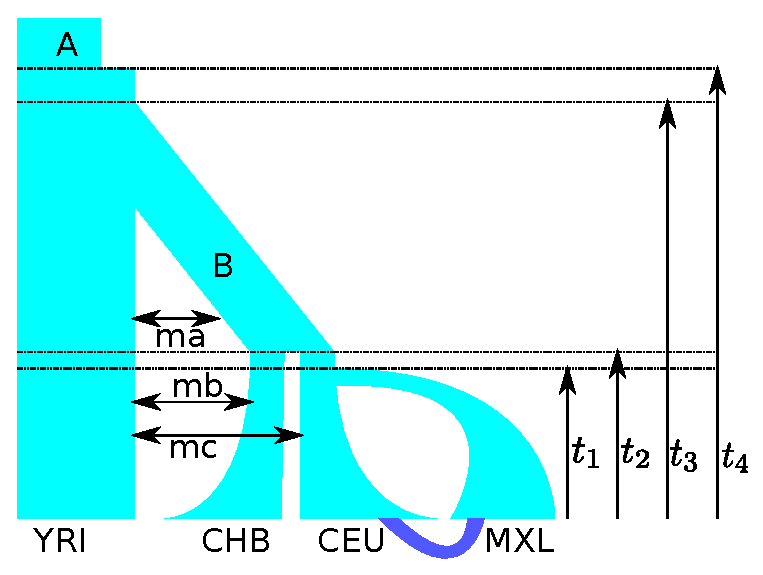
\includegraphics[width=.7\textwidth]{popModelLabel} 
\end{center}
\caption{A model of human demographics.}\label{fig:hard}
\end{figure}

The first pastward event is the MXL population joining the CEU population. We
assume that this happens 1600 generations into the past. The $t_1$ time is
therefore $1600/(4N_e)=1600/40000=0.04$. This is a deme joining event pastward,
so we add the following to our command line.
\begin{verbatim}
-ej 0.04 5 3
\end{verbatim}
Nothing else changes so that's all that's required. 

\subsubsection*{Second Event Pastward}

The second event is the joining of the CHB deme with the CEU demes. We set this
to be 2000 generations into the past so $t_2=0.05$. However, this time migration
changes as does population size. We also note that there is no longer any
exponential growth. We set the B population to  have the size of YRI, and 
the migration rate $ma$ is 12. Thus, we add
\begin{verbatim}
-ej 0.05 3 2 -en 0.05 2 .5 -em 0.05 1 2 12 -em 0.05 2 1 12 
\end{verbatim}
The {\tt -en} switch sets the growth rate to zero, so we do not need to use any
{\tt -eg} switch. 

\subsubsection*{Third Event Pastward.}

We have come to the last population merger. This happens 6000 generations
into the past. There is nothing else to set in this case, so we have.
\begin{verbatim}
-ej 0.15 2 1
\end{verbatim}

\subsubsection*{Last Event}

Finally, we have a  bottleneck 8000 generations ago where the population was
reduced to half its nominal value. The last option to add is.
\begin{verbatim}
-en 0.2 .5
\end{verbatim}

\subsection{Complete Command Line \& Selection}
The complete command line is therefore
\begin{verbatim}
>msms -N 10000 -ms 80 1000 -I 4 20 20 20 20 0 -t 100 -r 100 1000 
-es 0 3 .5 -ej 0 4 5 -g 2 10 -g 3 100 -g 5 200 -n 2 .0 -n 3 2 
-n 5 11 -m 1 3 5 -m 3 1 5 -m 1 2 2 -m 2 1 2 -ej 0.04 5 3
-ej 0.05 3 2 -en 0.05 2 .5 -em 0.05 1 2 12 -em 0.05 2 1 12 
-ej 0.15 2 1 -en 0.2 .5
\end{verbatim}
We claim there is selection in the CEU deme only and that standing variation was
initially zero with a medium forward mutation rate at the beneficial locus. We only
have to add the following.
\begin{verbatim}
-SI 0.05 5 0 0 0 0 0 -Sc 0 3 100 50 0 -Smu 0.1
\end{verbatim}
First, the {\tt -SI} option took the number of demes to be 5 despite the fact
that we ``joined'' one. This is because it still exists and we could set its
population size to a nonzero value. It is also important to note that the {\tt
-SI} option is the only option to work in forward time. That is, selection
starts at time 0.05 till the present. While the {\tt -Sc} option works
pastward, in this case from sampling time. Finally, we set the mutation rate to
0.1. 

\section{Trouble shooting}
Unfortunately things go wrong. Many of the times its is simply something wrong
with the command line options. Occasionally its a bug. Either way $msms$ tries as
hard as it can to tell you what is wrong. However this is harder than it looks
and often the error message can be cryptic or even misleading. This is a area
that is constantly improving so ensure you have the latest release. 

Often $msms$ puts out a lot of error messages. This is to make it easier for us
to pinpoint bugs when people give bug reports. Generally however you only need to
pay attention to the first few lines or so and can safely ignore the rest.

\subsection{\tt has an incorrect number of arguments.}
This error comes up frequently. It has a number of causes and not all of them
are in fact the wrong number of arguments. Currently you should check if you do
in fact have the correct number of arguments and that all switch's are typed
correctly. Note that all switch's are case sensitive. 

The reason this error comes up even if you do have the correct number of
arguments is that the next switch is typed wrong. The parsing code then thinks
this switch it does not know about belongs to the previous switch. The following
is a example.
\begin{verbatim}
msms 20 1000 -tt 5
\end{verbatim}
$msms$ does not identify the {\tt -tt} and the error message is:
\begin{verbatim}
 has an incorrect number of arguments.
options you tried was:
 20 1000 -tt 5 
Option help:
-ms  nsam replicates 
	Alias: 
	Required
	Sets sample size and replicates.
\end{verbatim}
You can see that under {\tt you tried was} is the {\tt -tt}. This tells you that
the switch is unrecognized. We are currently working on improving the parsing code to deal with this
situation better. So at least it gives a good error messages. 

\subsection{\tt Cannot condition on fixation times \ldots}
You have used the {\tt -SF} switch with a model that changes over time. This
does not work as $msms$ use a forward simulation for the allele frequencies not a
pastward process like the coalescent. There is no known pastward process for
selection trajectories for the general case. The only option is to use the {\tt
-SI} option instead.

\subsection{\tt Model does not permit full coalescent of linages.}
This is most frequently caused by having demes with samples without migration
between them. Since the lineages cannot migrate into the same deme, they cannot
coalesce and the simulation would run forever. In this case $msms$ has detected
this situation and has thrown an error. 

Generally any situation where lineages cannot coalesce should give this error.
However it is often hard to detect and may just run at 100\% CPU, never running
out of memory or finishing. 

\subsection{Out of Memory Errors}
Sometimes an out of memory errors is a indication that something else is wrong.
A common cause is when conditioning on fixation in a case where the beneficial
allele will never fix. The forward simulation will just run forever, or until it runs out
of memory. It is important to eliminate this case first before increasing the
memory available. 

However there are situations where one really does run out of memory and
increasing the memory available to $msms$ will solve the problem. The first thing
to know is that by default $msms$ will not try and just use all the memory of
your system but will give a out of memory error if it needs more than 256
megabytes of ram. Most modern systems have much more than this. It is easy to
tell $msms$ to use more, but this must be done by directly invoking java like
so.
\begin{verbatim}
java -Xmx500M -jar lib/msms.jar
\end{verbatim}
This is assuming that you are in the msms directory. This increases the ram
available to 500 megabytes. Generally setting this as high as all your ram my not
be a good idea. As once $msms$ uses all that ram, your computer could become so
slow that appears to be frozen. 

\subsection{Help My Problem is not here}
Please submit a bug report to the mailing lists {\tt
ms2-help@lists.sourceforge.net}. Remember to include the full command line you are
using. 

\section{Performance}

In this section, we demonstrate the current performance of the code with and
without selection and relative to ms. This should give some idea of what
parameters tend to dominate performance when using selection. 

Unfortunately, there are a lot of parameters that can affect performance and
details are important. We do not present a full study here, but merely use some
simple examples to illustrate general trends. We should also note that
different hardware will also perform differently, and different environments
such as operating systems can have an effect. Importantly, the version of java
used can have a big impact on performance of $msms$. Generally, the latest
version should be used as it includes the latest optimizations. For example Java
1.6.0u12 was about 10\% to 20\% faster than Java 1.6.0. Also, if one is running
on a 64bit machine, the 64bit version of java should be used.

\subsection{Introduction}
Performance of $msms$ is considered important, but not at the expense of
correctness. Because this is a selection simulator, the methods that work best
for reasonable parameter ranges under selection can be less optimal for other
cases. If such trade-offs occur, we have tried to optimize the code to improve
run times for parameter ranges where simulations are generally slow (in
particular, large recombination rates), even if this comes at the expense of
somewhat longer run times for parameter sets where simulations are very fast
anyway.  Hence, in some cases $ms$ will be faster than $msms$ for neutral models,
in particular with low recombination. 

All times were
collected on an AMD64 X2 Dual Core Processor 6000+, using Sun Java 1.6u18 64bit
and gcc 4.2.3 ruining Linux. $ms$ was compiled with a -O3 compiler option.

\subsection{Neutral models}

Lets first consider neutral models and compare with $ms$. The results for
representative parameter sets are shown in table \ref{tableMSvrsMSMS}. We note
that while $msms$ is slower than $ms$ in some cases, this only occurs in
parameter regions where both programs are fast (10000 replicates under 1 minute).
In these cases programs that print out a lot of data to the screen, such as $ms$
and $msms$ are generally IO limited (first 4 rows). However once we increase tree
depth, recombination or both, $msms$ is faster than $ms$,  almost 6 times faster
for one example. For long sequence lengths and for migration histories that
result in deep trees, $msms$ is a good choice even with neutral models.

These results also show which factors influence run times most strongly. Its
clear from table \ref{tableMSvrsMSMS} that recombination has by far the biggest
influence. This is even more true when selection is also considered. Migration also has
some influence on performance. However, the primary reason is that the deeper
tree results in more recombination events.

\begin{table}[htp]
\rowcolors{1}{white}{lightgray}
\begin{center}
\begin{tabular}{|c c c c| c c| c|}
\hline
$n$ & reps & migration & $\rho$ & $ms$ time & $msms$ & ratio \\
\hline \hline
100 & 10000 & - & 10 & {\bf 14.6} & 19.9 & 0.73 \\
100 & 10000 & 1 & 10 & {\bf 33.9} & 46.1 & 0.74 \\
100 & 10000 & - & 100 & {\bf 92.1} & 139.4 & 0.66 \\
100 & 10000 & 1 & 100 & 424.4 & {\bf 422.7} & 1.0\\
\hline\hline
100 & 1000 & - & 500 & 222.5 & {\bf 167.9} & 1.325 \\
10 & 1000 & - & 500 & 95.0 & {\bf 28.2} & 3.33 \\
10 & 1000 & 1 & 500 & 742.1 & {\bf 125.9} & 5.9 \\
10 & 1000 & - & 1000 & 495.0 & {\bf 94.0} & 5.27 \\
\hline
\end{tabular}
\end{center}
\caption{Performance of $ms$ compared to $msms$ for different parameters. The
number of recombination sites was 10000 and $\theta=10$. Cases with migration
have 2 demes with an equal number of samples from each. Times were collected on
an AMD64 X2 Dual Core Processor 6000+, using Sun Java 1.6u18 64bit and gcc
4.2.3. $ms$ was compiled with a -O3 compiler option. Times are in seconds. We
note that $msms$ does very well with deeper trees and high recombination. However $ms$ is still faster for low 
recombination rates. } 
\label{tableMSvrsMSMS} 
\end{table}

\subsection{Selection Performance}

Selection influences performance in a number of different ways. Principally, the
forward simulation step needs both CPU time and memory to construct. The
coalescent simulation is also slower because it must condition on frequency
trajectory. Finally, selection can have a large influence on the expected depth of the tree.

Results for selection are shown in table \ref{tableSelection}. For these
comparisons, we use the same set of parameters as for table \ref{tableMSvrsMSMS}.
The first result is that with high selection the run times can in fact be less
than in the neutral case. This can be understood by realizing that a large part
of performance is dominated by recombination and that high levels of selection
result in short coalescent trees at the selected locus. There are thus less
recombination events. High selection is also faster for the forward simulation as
a sweep takes less generations and the forward simulation can use less memory and
CPU cycles.

Table \ref{tableSelection} also shows that run times increase substantially if
selection strength is reduced. This is dramatic for $\alpha=10$, where
simulations  take over 6 times longer than under neutrality However, migration
does not influence the performance under selection more than under neutrality,
and we note that, overall, the performance is still similar to the neutral case.
Generally, recombination is again the dominant factor affecting
run times.


From these results, we can conclude that it is reasonable to simply add
selection to whatever demographic scenario one wishes to study. The performance
is comparable to neutral evolution for the most part. 

\begin{table}[htp]
\rowcolors{1}{white}{lightgray}
\begin{center}
\begin{tabular}{|c c c c|c c|c c|c|}
\hline
$n$ & reps & $m$ & $\rho$ & $\alpha$ & $N_e$ & neutral & selection & ratio \\
\hline \hline
100 & 10000 & - & 10 & 100 & 10000 & 19.9 & 32.7 & 0.62 \\
100 & 10000 & - & 10 & 1000 & 10000 & 19.9 & 12.6 & 1.58 \\
100 & 10000 & - & 10 & 1000 & $10^5$ & 19.9 & 35.5 &  0.56\\
100 & 10000 & - & 100 & 1000 & 10000 & 139.4 & 147.3 &  0.94\\
100 & 10000 & 1 & 100 & 1000 & 10000 & 422.7 & 452.9 &  0.93\\
\hline\hline
10 & 1000 & - & 500 & 1000 & 10000 & 28.2 & 21.3 &  1.32\\
10 & 1000 & - & 500 & 1000 & 10000 & 28.2 & 21.3 &  1.32\\
10 & 1000 & - & 500 & 1000 & $10^5$ & 28.2 & 23.9 &  1.18\\
10 & 1000 & 1 & 500 & 1000 & $10^5$ & 125.9 & 105.6 &  1.19\\
10 & 1000 & 1 & 500 & 100 & $10^5$ & 125.9 & 190.7 &  0.66\\
\hline \hline
10 & 1000 & - & 500 & 10 & $10^5$ & 28.2 & 194.1 &  0.15\\
\hline
\end{tabular}
\end{center}
\caption{Performance with selection. We use the same parameters as for
table \ref{tableMSvrsMSMS}. In all cases, we are conditioning on fixation at
sampling time ({\tt -SF 0}), and do not consider recurrent mutation at the
selected locus. Note that large selection improves performance compared to the
neutral case. This is because the tree is shorter and fewer recombination
events occur. Note that recombination is still the dominant. }
\label{tableSelection}
\end{table}

\section{Validation and Testing}

A small testing program is also included. This is used to test for regressions
and bug discovery. Currently, we compare the mean and standard deviation of some
summary statistics to other well-established programs with different options.
The summary statistics we use are average tree length, tree height, and
segregating sites and singletons. These are good at discriminating errors in the
code while being quick to calculate. For example if the tree height statistic
matches, but the segregating sites do not, we can assume that there is some bug
in the mutation code.

The tests are not rigorous statistically speaking. Currently, more statistically
sound testing is done with R and is difficult to automate. However, despite the
fact that these simple tests are not rigorous and perhaps some statistics appear
redundant, they have been shown to discriminate whenever more thorough tests
have failed. That is for cases where full statistical tests fail, these simple
tests also fail.

It is important to note that the tests are probabilistic in nature. Therefore,
we expect test failures by random chance alone. This becomes more pronounced with
more tests due to multiple testing. Several executions of the testing
program should however result in different failures or complete passes,
assuming no bugs have been introduced. 

In order to run the tests, there is a script in the bin directory called {\tt
simpleTest} that works on both Mac and Linux. Otherwise on all platforms,
inside the $msms$ directory the following will also invoke the test program:
\begin{verbatim}
>java -cp lib/msms.jar at.mabs.testing.BasicTests
\end{verbatim}



\bibliographystyle{applicationNote/natbib} 
\bibliography{applicationNote/Bio} 

\end{document}











